\documentclass[../thesis-main.tex]{subfiles}

\begin{document}
\label{ch:litreview}
  \begin{quote}
   \emph{In this section, the relevant background information is given. This starts with a brief outline of the function and structure of the heart, ranging from the high order organisation of the heart into functional compartments, down to the cellular level. Further details are then given on the physiological aspects of some of the subcellular components of cardiac tissue. The evolution of computational models to describe the electrical activity of the heart is charted briefly, with special attention given to models specifically used in this thesis. Variation is then described, both in experimental and physiological measurements, and how this variation has been addressed in computational models. Then the pathological condition of isch\ae mia will be described, and the computational efforts to model this outlined.}
  \end{quote}


 \section{Cardiac Physiology}
 \label{sec:physiology}
 At the most general level, the heart serves as a pump to transport blood around the body to deliver nutrients and remove waste products. It does this by rhythmic, organised contraction---the rate of this contraction varies depending on species, age, condition of the heart and the activity being undertaken by the organism.
 
 \subsection{Structure of the Mammalian Heart}
 \label{subsec:heart-structure}
 \begin{figure}
  \centering
  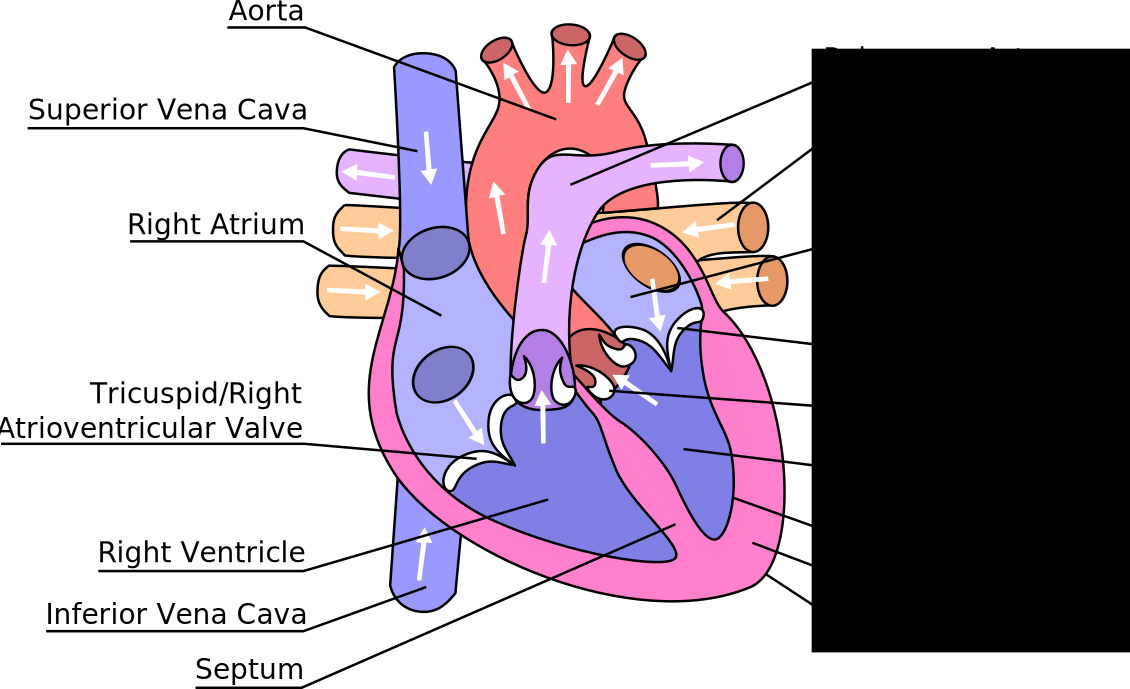
\includegraphics[width=0.75\textwidth]{heart_labels}
  \caption[Structure of the mammalian heart]{Diagram of the longitudinal cross-section of a mammalian heart. The direction of blood flow is shown by white arrows, and all major structural components are labelled.}
  \label{fig:heart-structure}
 \end{figure}
 Fig.~\ref{fig:heart-structure} shows the anatomical structure of the mammalian heart---while the size obviously varies widely between mammals, the overall architecture remains constant. It is split into two halves, left and right, by a muscular wall called the \emph{septum}, and then further subdivided into two chambers, the larger, lower chamber being a \emph{ventricle}, and the smaller, upper chamber called an \emph{atrium}.
 
 The passage of blood through the heart follows thus: firstly, deoxygenated blood from the body enters the heart via the superior and inferior/posterior \emph{vena cava}, with superior and inferior representing whether the blood comes from the upper or lower half of the body respectively. Via this channel, it enters the \emph{right atrium}. Passing through the \emph{tricuspid valve} (also known as the right atrioventricular valve), the blood enters the \emph{right ventricle}, where it is then pumped via the \emph{pulmonary artery} to the lungs, where it is oxygenated. The blood returns to the heart via the \emph{pulmonary vein}, entering the \emph{left atrium}, before moving through the \emph{mitral valve} (also known as the left atrioventricular valve) into the \emph{left ventricle}. The blood is then pumped via the \emph{aorta} to the rest of the body. The valves in the heart serve to ensure the flow of blood is always in the correct direction.
 
 The walls of the heart are mostly composed of muscular tissue known as \emph{myocardium}. The thickness of the myocardium is not constant throughout the heart, being thickest in the left ventricle, which requires the greatest force of contraction to pump the blood from the heart to the rest of the body. The myocardium can be split into three different regimes, as labelled in italics in Fig.~\ref{fig:heart-structure}: the \emph{epicardium} is the outermost layer of the myocardium, the \emph{midmyocardium} is the middle layer, and the \emph{endocardium} is the innermost layer. The cells composing these different layers possess different electrophysiological properties; the differences, and the consequences, will be expanded upon in \S\ref{subsec:electro-prop}.
 
 \begin{figure}
  \centering
  \begin{subfigure}[b]{0.45\textwidth}
   \centering
   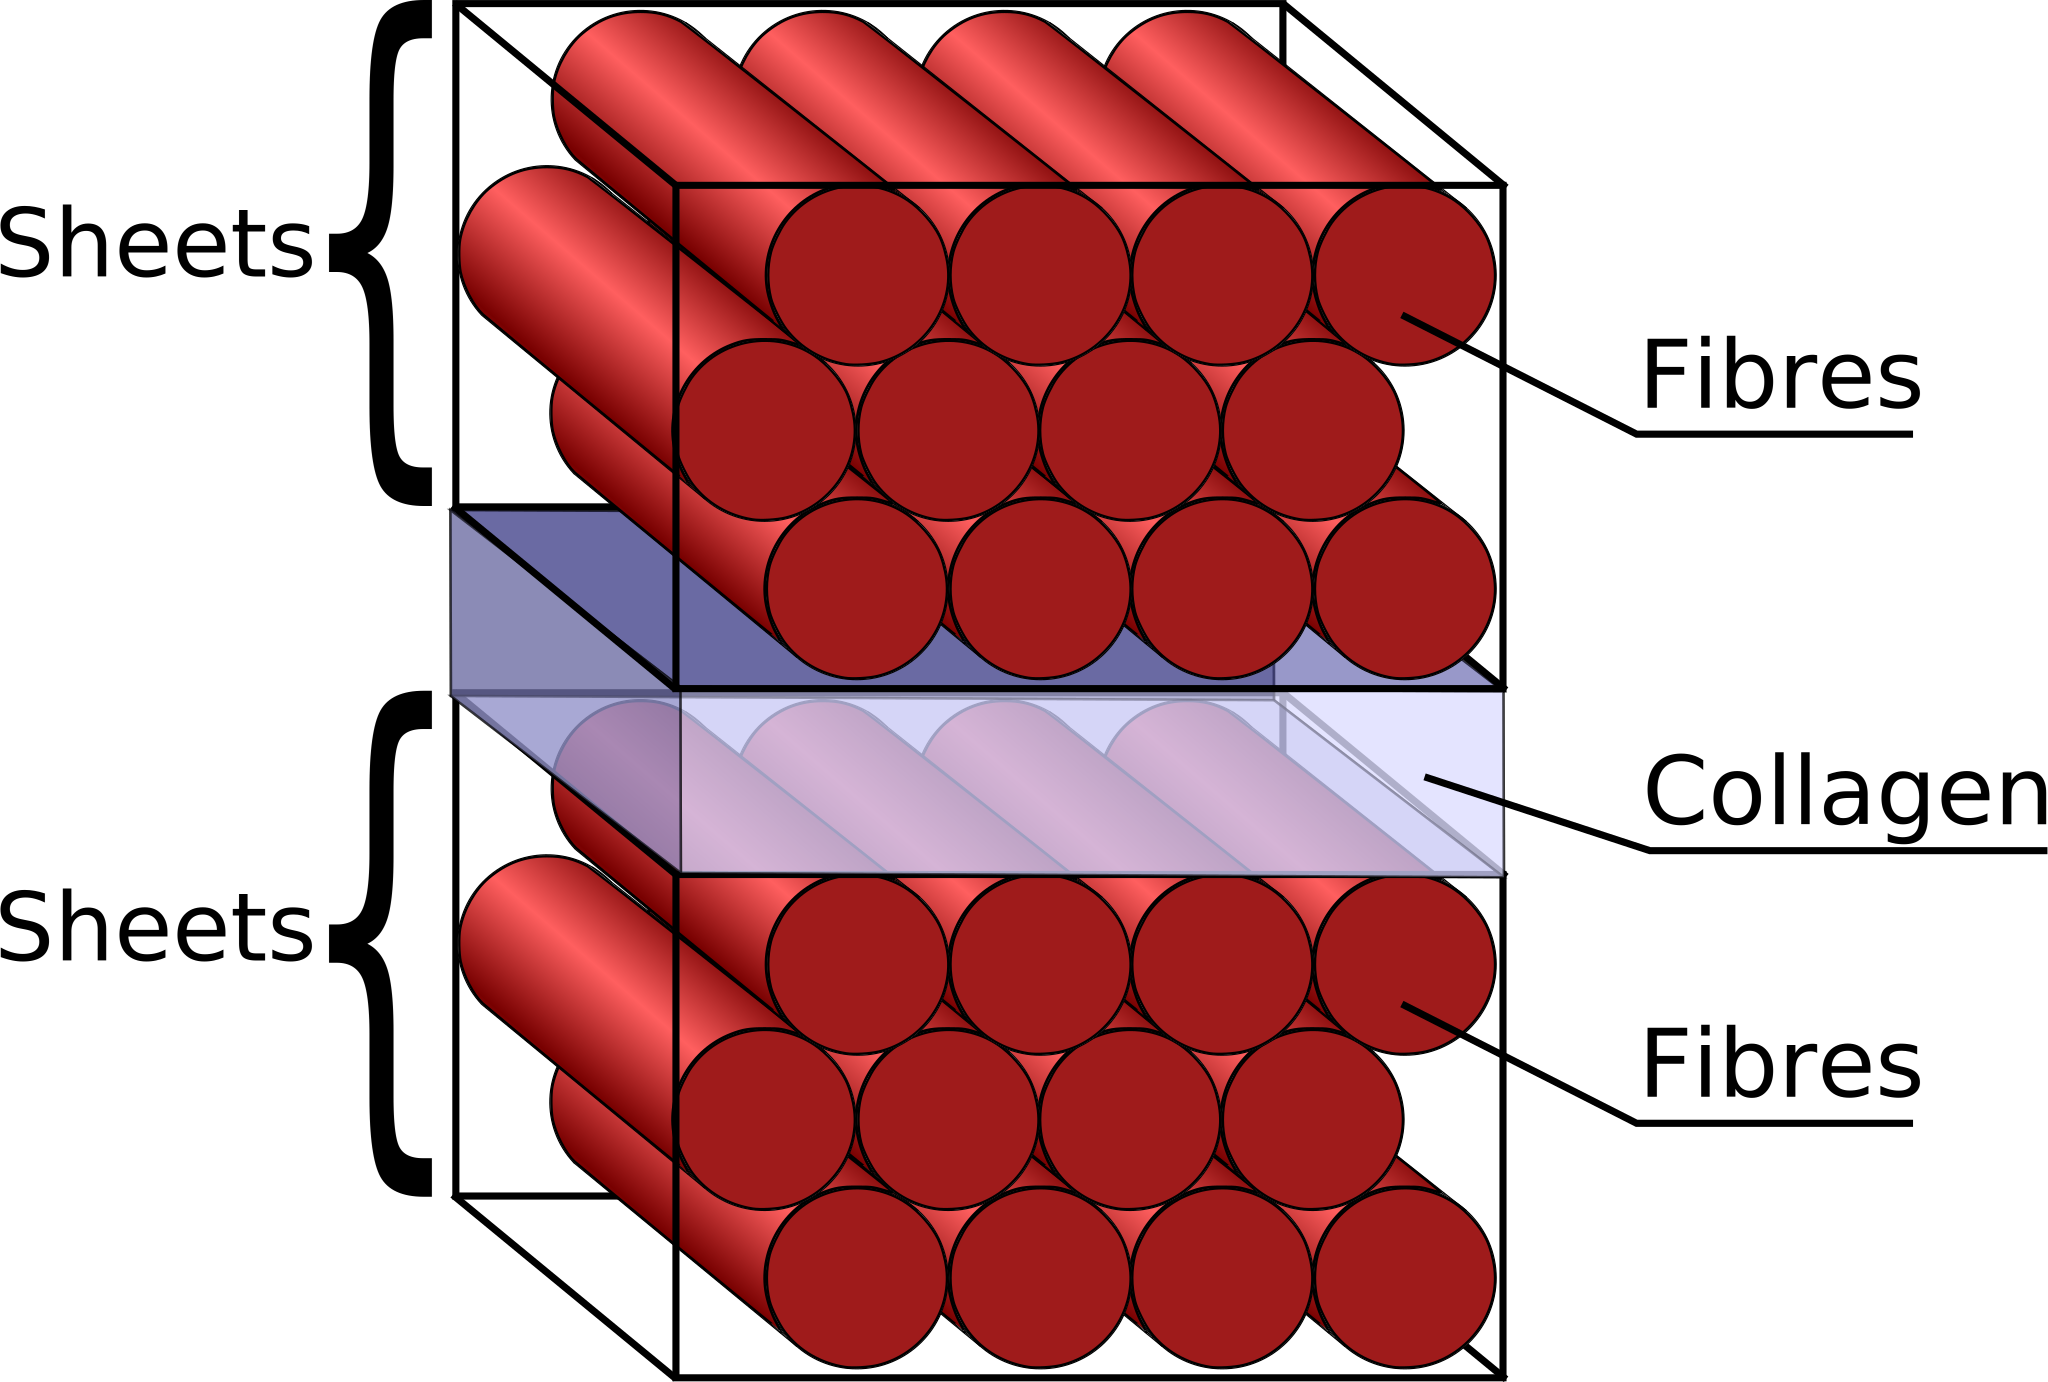
\includegraphics[width=\textwidth]{myocytes}
   \caption{Schematic}
   \label{subfig:myocyte-diagram}
  \end{subfigure}
  \begin{subfigure}[b]{0.45\textwidth}
   \centering
   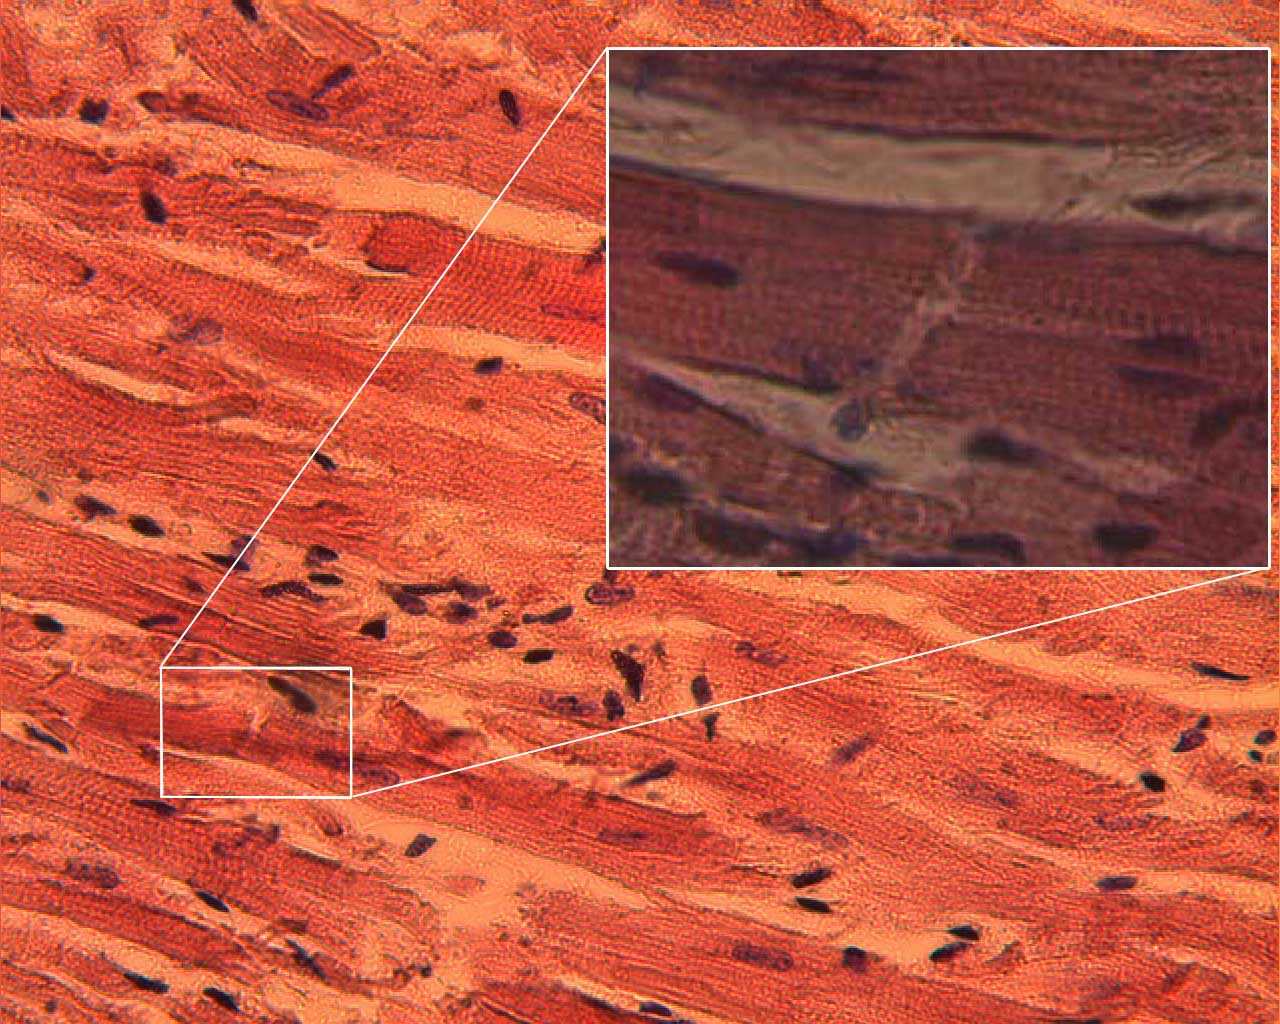
\includegraphics[width=\textwidth]{myocyte-image}
   \caption{Image}
   \label{subfig:myocyte-image}
  \end{subfigure}
  \caption[Structure of myocardial sheets and fibres]{(\ref{subfig:myocyte-diagram}) Schematic of the structure of myocardial sheets and fibres. (\ref{subfig:myocyte-image}) Image of cardiomyocytes demonstrating the interconnected nature of the individual myocytes into fibres.}
  \label{fig:myocyte-structure}
 \end{figure}
 
 The structure within the myocardium is shown in Fig.~\ref{subfig:myocyte-diagram}: it is composed of a series of sheets of tissue separated by collagen. The myocytes themselves lie longitudinally in these sheets to form fibres, with myocytes in the fibre direction connected to each other by intercalated discs (as opposed to skeletal muscle, which is composed of multinucleated fibres); this structure is seen in Fig.~\ref{subfig:myocyte-image}. One attribute of these discs is the presence of \emph{gap junctions}, which serve to electrically couple the myocytes by allowing ion flow between the two neighbouring myocytes in the fibre direction. This arrangement of the myocytes into electrically coupled fibres allows for coordinated contraction, and the fibrous structure allows the heart to twist as it contracts, leading to a more efficient pumping mechanism.
 
 The conduction pattern of the heart is key to the effective pumping mechanism---by controlling the sequence of electrical events in the heart, the sequence of conduction is similarly controlled. An outline of the conduction pattern of the heart is shown in Fig.~\ref{fig:conduction-pattern}. The sequence of activation starts amongst a group of self-excitatory cells at the top of the right atrium, called the \emph{sinoatrial node}. The action potential wave spreads from this node, causing the atrium to contract, before it reaches the \emph{atrioventricular node}---this is the only pathway for electrical excitation to pass from the atria to the ventricles. From the atrioventricular node, the excitation wave passes to the \emph{Bundle of His}, which conducts the electrical stimulus via the left and right bundle branches into the \emph{Purkinje system} near the bottom of the heart, which transmits the stimulus to the ventricular surface; as the stimulus has thus been transmitted directly from the atria to the bottom of the ventricles, the excitation wave thus spreads upwards through the ventricles, allowing the ventricles to contract from the bottom up as required.
 \begin{figure}
  \centering
  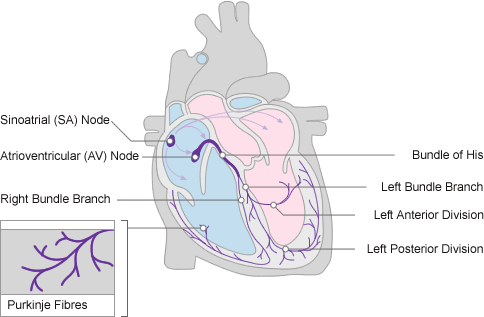
\includegraphics[width=0.8\textwidth]{cardiac_conduction}
  \caption[Pattern of electrical activation in the heart]{Schematic outline of the sequence of electrical activation in the mammalian heart. Image originally downloaded from www.nottingham.ac.uk on 10th December 2012.}
  \label{fig:conduction-pattern}
 \end{figure}
 
 \subsection{Electrophysiological Properties of Cardiomyocytes}
 \label{subsec:electro-prop}
 As previously stated, the main r\^ole of the heart is to serve as a pump to circulate the blood around the body. To do this effectively, it requires coordinated contraction, and this is achieved through the use of coupling the electrical activity of the heart of the mechanical activity (the details of this mechanism will be expanded upon in \S\ref{subsubsec:ecc}).
 
 Physically, cardiomyocytes are typically $10-20\mu$m in diameter, and $50-100\mu$m in length. They are cells bound by a lipid bilayer membrane, separating intracellular space (containing the cytoplasm, nuclei and other organelles) from the extracellular space. Embedded within the bilayer are various ion channel and transporters, which allow the membrane to be selectively permeable to various ions and other substances, and to regulate the flow of these ions as required. Thus, the intracellular space has a very different composition to the extracellular space, with the intracellular space containing a high and low concentration of potassium (\K) and sodium (\na) ions respectively; the reverse is true for the extracellular space. This concentration gradient is largely maintained by the \na-\K{} pump. These concentration differences are the main reason behind their being a potential difference set up across the cell membrane, referred to as the \emph{membrane potential} ($V_m$). At rest, due to the high \K{} and low \na{} in the cell,this potential is negative, though the magnitude varies depending upon the location in the heart; a cardiomyocyte in the ventricles typically has a resting potential ($V$\sub{rest})) of about $-80$mV, while the sinoatrial node has a resting potential of between $-50$ and $-60$mV.
 
 Electrically, the heart can be modelled with great success as an analogue to an electrical circuit \citep{Carmeliet2002}, where the lipid bilayer is represented as a capacitor, and the various ion channels and transporters that span the membrane are represented as resistors, which change their `resistance' depending on their state. By altering the resistance of these channels, ion flow across the membrane is permitted via an ionic current, which changes the membrane potential---the characteristic change in membrane potential associated with, and causing, a contraction is referred to as the \emph{action potential} (AP).
 
 It is a point of nomenclature that an `inward' current represents the movement of positive ions from the extracellular to the intracellular space, and an `outward' current is the reverse. This definition is based on the movement on electrical charge, and not on the movement of ion flow.
 
 \begin{figure}
  \centering
  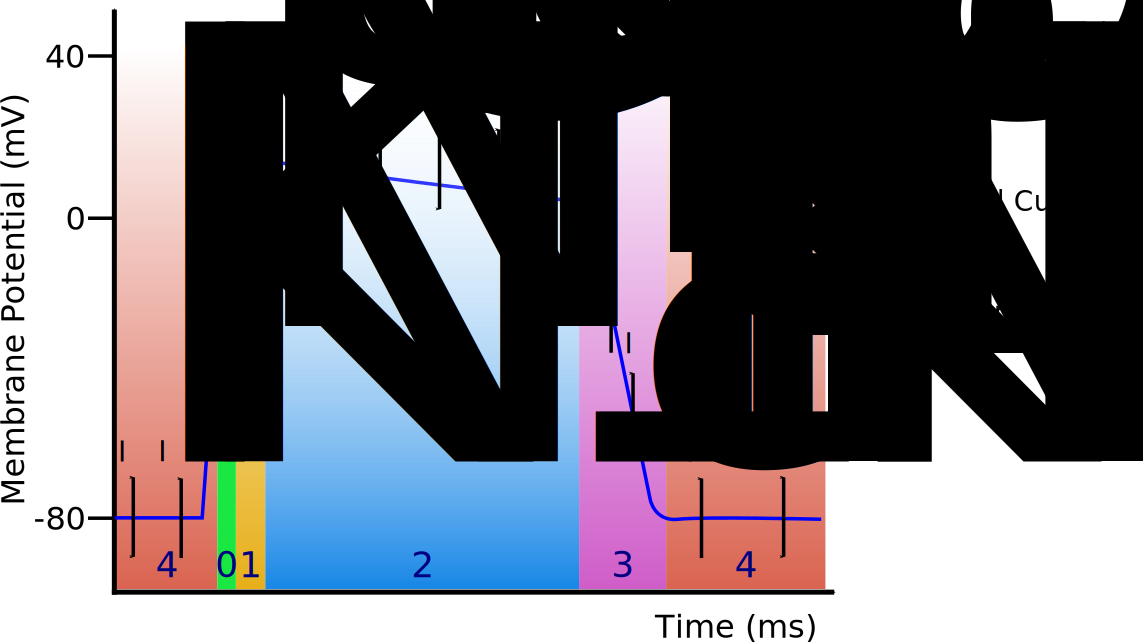
\includegraphics[width=0.8\textwidth]{ap-structure-full}
  \caption[Schematic of a cardiac AP]{Schematic of a ventricular cardiac AP, with the different `phases' of the AP shown, and which key currents are involved in each phase. Upward arrows represent outward currents, inward currents represent inward currents, and double arrows represent exchangers, \idest, where current moves in both an inward and outward direction.}
  \label{fig:ap-structure}
 \end{figure}
 An example of an action potential, showing the different `phases', is shown in Fig.~\ref{fig:ap-structure}. The AP is considered to consist of 5 different phases:
 \begin{description}
  \item[Phase 4:] The resting phase. For ventricular and atrial cardiomyocytes, this phase is marked by a relatively constant value for $V_m$. The negative resting potential is largely achieved by the inwardly rectifying potassium current (\ikix{}) remaining open during this phase. For pacemaker cells, \ikix{} is absent, and thus the resting phase is actually a period of slow depolarisation, until $V_m$ reaches the threshold value for phase 0.
  \item[Phase 0:] Period of rapid depolarisation that marks the start of the AP. It is initiated by $V_m$ reaching a threshold value which causes the \ina{} current to activate, causing a rapid influx of \na{} into the cell.
  \item[Phase 1:] Transient repolarisation. The \na{} channels rapidly deactivate, and the transient outward current, \ito{}, results in a period of rapid, partial repolarisation. Depending on the strength of this current, this repolarisation may be to the extent that there is a `notch' in the AP. For example, there is a notch in the AP for ventricular epicardial cells, but no notch for ventricular endocardial cells.
  \item[Phase 2:] Plateau phase. The membrane potential is sustained at a relatively constant level by a balance of calcium (\ca{}) influx via the L-type calcium current (\ica{}), and potassium efflux, through the rectifier \K{} currents (\ikr{} and \iks{}).
  \item[Phase 3:] Repolarisation. The L-type \ca{} current channels close, while the \iks{} channels remain open, allowing continuing \K{} efflux resulting in a repolarisation of the cell to the original resting potential. \ikix{} opens during this phase, to remain open during phase 4 to maintain a steady resting potential. 
 \end{description}
 It should be noted that the above is only an outline---the AP is the result of a complex series of interactions between different currents and channels opening and closing in response to the membrane potential and other inhibitory and activating factors.
 
 \subsubsection{Excitation-Contraction Coupling}
 \label{subsubsec:ecc}
 Arguably, the complex electrical activity of the AP just described exists for the sole purpose of ensuring the heart acts as an effective mechanical pump. As such, the linking of the electrical activity of the heart to its mechanical contraction is vital, as is referred to as \emph{excitation-contraction coupling} (ECC). What follows is a brief summary of the mechanism of this link (the reverse side of this mechanism, termed mechanoelectric feedback, shall not be discussed here).
 
 For ECC, the cell may be decomposed into units called calcium release units (CRUs), also known as dyads \citep{Cleemann1998}. These CRUs are spread roughly evenly throughout the cell to allow for a uniform action throughout---the number of CRUs in the cell has been estimated to be between 10,000 and 100,000 \citep{Cleemann1998,Greenstein2002}. Anatomically, the CRU may be considered to be a section of the cell containing a section of the cell membrane, with some L-type \ca{} channels, and a section of the sarcoplasmic reticulum (SR). The primary r\^ole of the SR is to sequester and release \ca{} via ryanodine receptors (RyRs) when the required stimulus is given. This stimulus is the rise in local concentration of \ca{} precipitated by the opening of the L-type \ca{} current channels, and is termed \emph{calcium-induced calcium release}. The result is that a great deal of \ca{} is released into the cytosol of the cell during phase 2 of the AP. The reason this is vital for ECC is due to the interaction between \ca{} and the contractile units of the cell, called the sarcomere. When the cytosolic concentration of \ca{} (\cai{}) rises, the free \ca{} binds to a part of the contractile machinisms of the cell, which then removes the inhibition between the two critical contractile parts of the mechanism, allowing contraction to take place. Subsequently, the \ca{} released from the SR is recovered by the sarco/endoplasmic reticulum \ca{}-ATPase pumps \citep{Franzini-Armstrong2005}.
 
 \subsubsection{Ion Channel Mechanics \& the Repolarisation Reserve}
 \label{subsubsec:channel-mechanics}
 As stated previously, the potential difference across the membrane is maintained and altered by the action of various membrane-bound proteins, which can be classed as either \emph{channels}, \emph{pumps} or \emph{exchangers}. Most of these proteins present ion-specific openings through the membrane, though different channels have different degrees of selectivity. Most of these channels are also controlled by, amongst other things, the membrane potential itself \citep{Bezanilla2000}. The membrane potential causes a conformational change in the ion channel protein, causing it to `open' or `close', that is to allow ions to be conducted through it or not.
 
 These ion channels are discrete molecular entities, and thus the conformational changes that lead to their open/close state are stochastic; the effects of this stochasticity are discussed in greater detail in \S\ref{sec:param-var}. However, each type of ion channel possesses its own range of attributes, such as the time it takes to inactivate, the time it takes to reactivate, its permeability to different types of ions, and its susceptibility to other gating factors. For the channels examined in this thesis, a brief summary of their action and relevant physiological properties is given; further details are given in the Appendix. A comprehensive summary of the physiological properties is given in \citet{Carmeliet2002}.
 
 \section{Computational Cell Models}
 \label{sec:cell-models}
 
 \section{Variation}
 \label{sec:param-var}
 
 \subsection{Experimental \& Physiological Variation}
 \label{subsec:experimental-var}
 
 \subsection{Computational Modelling of Variation}
 \label{subsec:comp-var}
 
 \section{Isch\ae mia}
 \label{sec:ischaemia}
 
\end{document}
